\section{监考怎么做}

\subsection{如何参加}
全奖博士如果没有做满规定的TA时长,这时候学院就会给你安排监考。监考一学期只有两次,期中考和期末考。由于近两年疫情,很久没有线下考试啦。

遇到考试较多,教职工和全奖博士不够用的情况,非全奖的博士也可以报名做监考员。具体的方式就是等待学校发邮件邀请,会有一个链接,让你点进去选择心仪的时间。选完之后过几天就可以在e-bridge上查看具体的监考安排啦。

监考的工资单价,2022年是60元一个小时,准备工作比较少,监考途中基本也就是走一走,相对轻松,对于非全奖是不错的挣钱方法。

\subsection{具体怎么做}
首先学校有监考的培训,在\textit{Teaching Assistant (TA) Training Programme}为题的邮件里的Assessment and invigilation那一项就是,或者是在你的LMO里翻一下。如果一次都没去过,可以考虑去听一下大致的流程。

一个考场的监考分为senior invigilator(教职工)和invigilation assistant(博士生)。

我总结下来监考的流程是这样
\begin{enumerate}
    \item 上面说的监考培训,虽然不是每次都必须听,但按照惯例,是在每学期培训的时候发[监考员工牌]。监考时必须佩戴,监考完必须还回学校。所以,即使不想听也至少要跑一趟去领你的工牌。如果更懒(比如我),一般让办公室其他要监考的同学代领(一般是办公室派一个人把整个办公室的都领回来)。
    \item 在ebridge上查到自己的监考安排,如下图
        \begin{figure}[H]
            \centering
            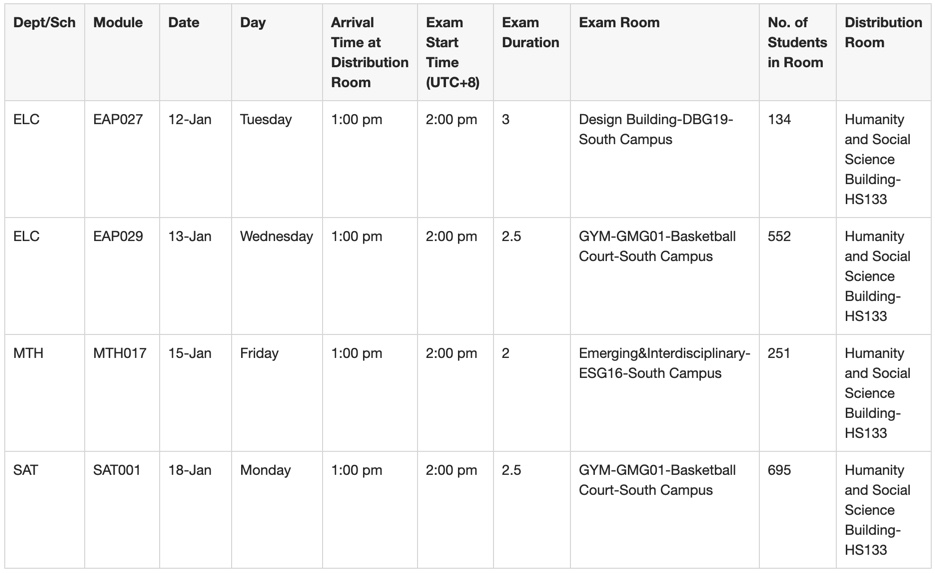
\includegraphics[width=0.5\columnwidth]{author-folder/Kai.Wu/invigi-table.jpg}
        \end{figure}
    \item 监考第一部分:考前准备。开考前,注意上面表格里的两列:"Arrive Time at Distribution Room" 和 "Distribution Room",在指定时间,提前去签到并领取试卷。然后会拿到MCQ card、答题册、考场名单、小白卡、黏土等资料,拿到考场去
    \item 到了考场,第一件事是粘贴资料。考生名单里,有一份按学号排序的是用来贴在门上的,给学生找自己的座位(其他几份按座位排序的是给监考员自己拿着的)。把这一份资料每一页分开,用黏土贴到考场门上或者墙上。
    \item 然后开始分发答题册、答题卡。对照考生座次发。
    \item 一般一个考场会有多个监考。其他监考员来了过后,分一些发答题册、答题卡的任务给他们。然后,跟他们商量每个人负责的区域,每人负责一个区域的监考巡视、收资料等工作。
    \item 主监考(监考老师)会带着试卷来,然后帮老师发试卷。如果主监考在开考前20分钟还没到,需要联系监考员微信群里的老师催促。
    \item 开考15分钟前,必须所有资料(试卷、答题卡、MCQ等)发放完毕。考试前15分钟,让学生入场。
    \item 多个监考员在场时,一般每个入口留一个以上监考员查学生卡,没带学生卡或身份证的不准入场。其他监考员,可以在考场里走动,特别注意学生在开考前不许打开试卷册,如果发现需要立即制止。如果比较多,要让主监考警告学生。为防止丢失,学生的背包不要放到考场外,让学生只能放到考场最前面或最后面。
    \item 主监考宣布开考后,对于你负责的那个区域,记录迟到的学生。可以记录在你的监考名单上。
    \item 开考后,随便转悠,享受你作为监考员的权威。重点检查学生的随带物品,手上或纸条是否有小抄等。监考过程中,不可以看手机或者闲聊,需要观察学生是否有作弊现象。若遇到作弊的,需要当场指出,停止学生考试并在试卷上做出标记。
    \item 开考后30分钟,收小白卡(一张专门用来写姓名学号等信息的卡片)。收完过后,记录你的区域的缺考的学生。
    \item 如果有学生没带笔、铅笔、橡皮要借,问主监考如何操作。如果有学生要上厕所,需要监考员跟随过去(跟到厕所外就可以了,虽然貌似也不用提醒)、跟随返回。同一时间,原则上只能有一个学生上厕所。如果有第二个要去,需要考生等前一个回来。
    \item 最后就是考试结束,收所有资料,包括草稿纸(如果有)。学生必须要等你们收完了、点清数量无误,才能起身离开。
    \item 考完过后,统计到场、迟到、缺席等情况,让主监考记录在记录表里。最后,有两张纸需要所有监考员签字。有这两个签字 + 一开始的签到,才会成功记录你的工作。
    \item 然后就是say goodbye了。监考老师会拿走答题册、MCQ。你们需要把前面签字的两张纸和所有监考老师不要的资料(包括试卷、草稿纸等)拿回一开始签到的地方。如果这是你本学期最后一次监考,需要把你的监考工牌也还回去。
\end{enumerate}

\emptyline{}
最后分享一个我做了十几次监考过后自用的checklist

\begin{enumerate}
    \item 拿东西的时候看监考员人数,方便分区域
    \item 到考场贴座位表
    \item 跟老师确认
    \begin{enumerate}
        \item 收答题册按顺序?如果要,考试结束不要让学生传卷子,缺考的、提前交卷的也放在桌子上
        \item 贴?如果要,考试结束让学生贴
        \item 是否要记录上厕所和开始结束时间
        \item 缺考的怎么处理(小白卡、答题册 帮填信息,答题册写Absent)
    \end{enumerate}
    \item 拿到座位号先按监考员数量分区域,区域作用:除了收卷子都负责
    \begin{enumerate}
        \item 考前:发卷子,查看区域是否坐对了座位,看学生不要打开白色问题册
        \item 放学生:门口检查学生卡
        \item 0-30分钟:查看坐对座位,记录迟到
        \item 30分钟:记录absent,收小白卡。之后填写学生到场情况表
        \item 上厕所:记录上厕所的座位号、开始结束时间
        \item -15分钟:记录提前交卷座位号、人数
    \end{enumerate}
    \item 结束前:提醒老师让学生粘answer booklet
    \item 结束后:按顺序收answer,清点自己收的部分,拿到一起后再随机清点一部分
    \item 分块列表:人数、缺勤、提前交、剩余、特殊
\end{enumerate}


\begin{figure}[H]
    \centering
    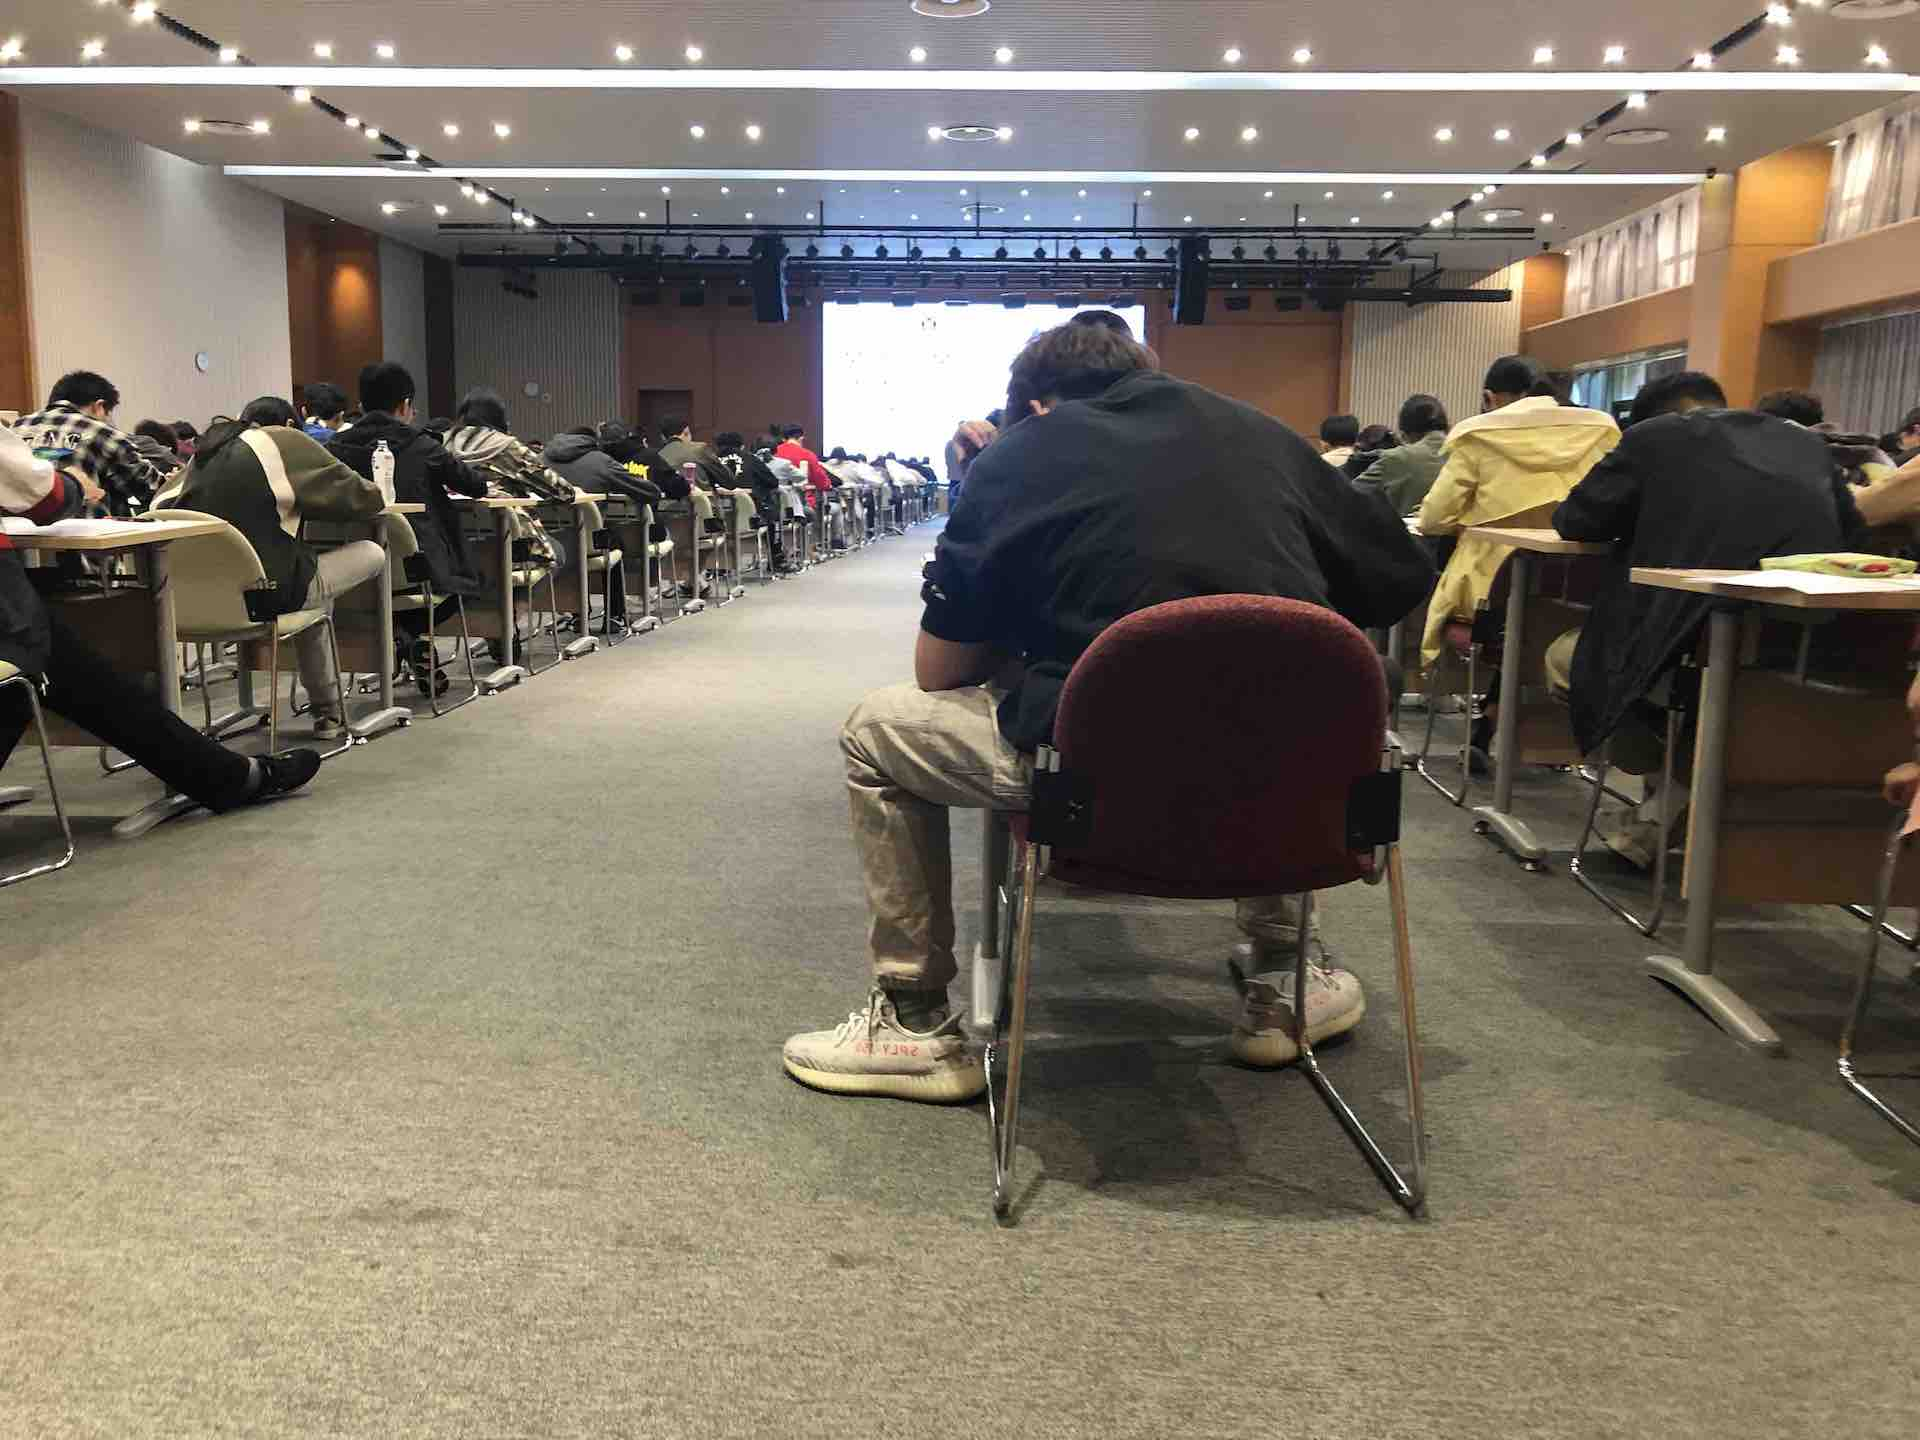
\includegraphics[width=0.9\columnwidth]{author-folder/Kai.Wu/invigilation.jpg}
    \caption{2020年11月15日,CB楼G层某考场,监考中}
\end{figure}

\begin{flushright}
(2022年10月22日 by Kai Wu)

(major update: 2022年12月30日 by Yue Zhou)
\end{flushright}

% \begin{figure}[H]
%     \centering
%     \includegraphics[width=0.5\columnwidth]{author-folder/Kai.Wu/}
% \end{figure}


% \usepackage[export]{adjustbox}

% \item 
% \begin{minipage}{0.3\textwidth}
%     文字
% \end{minipage}
% \begin{minipage}{0.63\textwidth}
%     \begin{figure}[H]
%         \includegraphics[width=0.4\columnwidth, right]{author-folder/Kai.Wu/}
%     \end{figure}
% \end{minipage}

% \input{author-folder/Kai.Wu/.tex}
